\documentclass[11pt,a4paper]{article}
\usepackage[margin=2.4cm]{geometry}
\usepackage{amsmath,amssymb}
\usepackage{booktabs}
\usepackage{graphicx}
\usepackage{enumitem}
\usepackage{url}
\usepackage{tikz}
\usetikzlibrary{arrows.meta,positioning,fit}
\usepackage{algorithm}
\usepackage{algpseudocode}
\newcommand{\code}[1]{\texttt{#1}}
\newcommand{\HV}{\mathrm{HV}}
\newcommand{\IGD}{\mathrm{IGD}}
\usepackage{adjustbox}
\setlength{\emergencystretch}{3em}
\usepackage{natbib}
\begin{document}
\title{Supplementary material}
\date{}
\maketitle
\section{Extended background and settings}
\subsection{How it was done before language models}
Early work on hardware-aware network design includes multi-objective structure search with a modelled implementation cost \cite{smithson}, Bayesian optimisation of accelerator and network settings \cite{hernandez,reagen}, power- and memory-constrained hyper-parameter optimisation from GPU measurements \cite{hyperpower}, and search with latency measured on the target phone \cite{netadapt,mnasnet}. MnasNet put measured latency into a reinforcement-learning reward and needed about 4.5 days on 64 TPUv2 devices for roughly 8{,}000 sampled models \cite{mnasnet}. Later work reduced that cost mainly by removing per-candidate training. ProxylessNAS made latency differentiable through a prediction model and searched on the target task in 200 GPU-hours \cite{proxyless}. FBNet used an additive lookup table of operator latencies and 216 GPU-hours \cite{fbnet}. Once-for-All trained one large network once (about 1{,}200 GPU-hours) and then searched sub-networks for each device with an accuracy predictor and a latency table \cite{ofa}. ChamNet \cite{chamnet} adapted an existing efficient network with a genetic algorithm whose fitness came from a Gaussian-process accuracy predictor (built from 240 trained networks), an energy predictor and a lookup table of about $350{,}000$ operator latencies for a device; its authors report that, once these predictors exist, an architecture for a new platform or constraint takes minutes, and state the total cost as $O(m+n)$ rather than $O(mnk)$ for $m$ networks, $n$ platforms and $k$ constraints. In this recipe the saving comes from the evaluator; the search operator is a conventional genetic algorithm. MobileNetV3 \cite{mobilenetv3} combined a MnasNet-style search \cite{mnasnet} with layer-wise adaptation \cite{netadapt} and then improved the result by hand: its authors state that redesigning the expensive first and last layers and adding the h-swish nonlinearity lay outside the search space, and they call the best way to blend automated search with human intuition an open question.


\subsection{Search strategies: advantages and pitfalls}
A search needs a search space, a search strategy and a way to estimate performance \cite{elsken}. Reinforcement learning composes novel structures but trained every child: 12{,}800 architectures on 800 GPUs in the original work \cite{zoph17}. Regularised evolution is simple and ahead of reinforcement learning early in a search, but the two were similar at 20{,}000 models, at about 450 GPUs for 7 days \cite{real19}. Gradient-based search (DARTS) cut the cost to 1.5--4 GPU-days \cite{darts}, but its authors note that the search must be repeated and memory grows with the candidate set, and benchmark studies report it collapsing to a cell dominated by skip connections \cite{nb201,nats}. Weight sharing made evaluation cheaper still (0.45 GPU-days for ENAS \cite{enas}), at the price of weaker ranking: the Kendall correlation between supernet and true ranking was only $0.42$--$0.64$ in one study \cite{spos}. Surrogate-guided search trains only the candidates a predictor selects, with up to five times fewer evaluations than reinforcement learning \cite{pnas}. Random search has repeatedly been reported as a strong baseline in this literature \cite{zoph18,darts,lital}, and one study found that several state-of-the-art algorithms perform similarly to a random policy on average \cite{yu20}. The same literature documents weak evaluation practice: of 12 recent NAS papers, none were exactly reproducible \cite{lital}.


\subsection{How performance is estimated today}
Most of the cost reduction above came from cheaper performance estimation, not from smarter search. Tabulated benchmarks store the trained accuracy of every architecture in a space: NAS-Bench-201 holds $15{,}625$ cells \cite{nb201}, of which NATS-Bench lists about $6.5$ thousand as distinct topologies \cite{nats}. HW-NAS-Bench adds latency and energy for each cell on six devices, four measured on hardware (Edge GPU, Raspberry~Pi~4, Edge TPU, Pixel~3) and two estimated by simulators (Eyeriss, FPGA) \cite{hwnasbench}. Zero-cost proxies score untrained networks in about a second; adding one to random search, reinforcement learning, aging evolution or predictor-based search improved their search speed, by up to four times over the previous best result on NAS-Bench-101 \cite{abdelfattah}. A regressor fitted on a sample of trained architectures (boosted trees or a graph network) is how spaces of $10^{18}$ to $10^{21}$ architectures were made cheap to query \cite{nb301}. These tools have pitfalls. Tables exist only for small spaces; proxies are biased toward larger architectures \cite{nbsz}; a latency predictor's errors can change which models are Pareto optimal \cite{brpnas}; and conclusions from small tabulated spaces need not carry over to large ones. In NATS-Bench, random search trails regularised evolution on CIFAR-100 in the topology space, and on CIFAR-100 and ImageNet-16-120 in the size space \cite{nats}, and in the $10^{18}$--$10^{21}$ spaces of NAS-Bench-301 random search needs many times more evaluations than regularised evolution or HEBO to reach a comparable architecture \cite{nb301}.


\subsection{Unspecified details and the choices made}\label{sec:assumed}
\begin{table}[h]\centering\small
\caption{Choices not specified by the paper (all exposed in \code{configs/base.yaml}); these are the first things to vary in a sensitivity study.}\label{tab:assumed}
\begin{adjustbox}{max width=\linewidth}
\begin{tabular}{p{4.6cm}p{4.0cm}p{6.2cm}}
\toprule
Item & Choice & Rationale \\
\midrule
Initial population per niche & 5 random architectures & Algorithm~1 samples but gives no size \\
Children per Stage-2 call & 4 & $6\times10\times4=240$ proposals over 120 calls \\
Parents shown per prompt & $\le6$ (half newest, rest random) & Fig.~4 shows both ``last cycle'' and ``random from archive'' \\
Crossover probability $p_c$ & each child slot assigned crossover w.p.\ 0.5 & reconciles Sec.~4.1 ($p_c{=}0.5$) with App.~E (LLM decides) \\
Knowledge-base scope & one per niche & Stage-1 prompt contains the niche definition \\
Invalid / duplicate / out-of-niche proposals & discarded, no retry, counted & keeps the 120-call budget fixed \\
\code{latency\_limit} in prompt & omitted & never given a value \\
Temperature & 0.7 (not sent to Claude, whose current models accept no sampling parameters) & not stated \\
Predictor training set & 1{,}000 archs, validation labels & ``trained on a sample''; avoids test leakage \\
Accuracy for HV/IGD & NB201 200-epoch test accuracy & Table~2 reports the 94.37\% test optimum \\
Discovered set $S$ & final front of Algorithm~1 (chosen by predicted accuracy), re-scored with true accuracy & Algorithm~1 returns $P_{\text{final}}$ \\
HV/IGD normalisation & true-front min--max, $r=(1.1,1.1)$, HV as a ratio & paper reports $\HV\le1$ \\
Seeds & CIFAR-10: 10 for non-LLM runs, 3 for the local LLMs, 1 for the API LLMs; CIFAR-100: 3 & paper reports $\pm$ without a count; API runs limited by cost \\
\bottomrule
\end{tabular}
\end{adjustbox}
\end{table}


\subsection{Scope of what was run}
Table~\ref{tab:scope} states exactly which paper items were and were not reproduced. We report this explicitly because the API-based LLM runs are expensive and were limited to one seed; the two local models were run with three.
\begin{table}[h]\centering\small
\caption{Reproduction status by paper item.}\label{tab:scope}
\begin{adjustbox}{max width=\linewidth}
\begin{tabular}{p{4.3cm}p{2.3cm}p{8.1cm}}
\toprule
Paper item & Status & What was done \\
\midrule
Table 1 (niches) & reproduced & niche sizes computed from the benchmark \\
Fig.~2 (encoding), Fig.~3 (parameter clusters) & reproduced & example rows matched to the benchmark; Fig.~3 regenerated \\
Table 2 (selected architectures) & checked & 11/12 LLM-NAS points located in the benchmark (the main paper) \\
Table 3 (HV/IGD, 3 datasets $\times$ 6 devices) & \emph{one dataset} & CIFAR-10, all six devices (the main paper): GPT-4.1 and Claude Haiku~4.5, 1 seed each; DeepSeek-Coder-V2 and Qwen, 3 seeds each; Claude Opus~5.5 on Edge GPU only; five non-LLM controls, 10 seeds; CIFAR-100 and ImageNet16-120 not run with LLMs \\
Table 4 (search cost) & measured & tokens, calls and time recorded for the runs above \\
Table 5, Figs.~6--8 (ablations) & \emph{partial} & non-LLM methods (PEA, random sampling, NSGA-II, regularised evolution) on CIFAR-100, 6 devices, 3 seeds; the full-model and Synflow rows were not run \\
Figs.~1, 9 (exploration bias) & implemented, not run & \code{fig1\_bias} experiment exists \\
Sec.~4.4, Table 6, Fig.~5 (ViT) & not reproduced & needs an AutoFormer supernet and A6000 timing \\
Baselines (FairNAS, PRP-NAS, LLMatic, DARTS) & quoted & GPU-days of training each \\
\bottomrule
\end{tabular}
\end{adjustbox}
\end{table}


\subsection{Ablation on CIFAR-100 (paper's Table 5)}
The paper reports that removing the LLM operator (PEA) lowers average HV on CIFAR-100 from 0.978 to $0.843\pm0.075$. We could only run the non-LLM variants. With our normalisation, PEA achieves $0.946\pm0.031$ averaged over the six devices (three seeds each), and uniform random sampling within niches $0.931\pm0.047$; NSGA-II and regularised evolution with the same predictor and 270 evaluations reach 0.959 and 0.962 (Table~\ref{tab:abl}, Figure~\ref{fig:abl}). Our PEA is $\approx0.10$ above the paper's PEA, a gap as large as the one the paper attributes to the LLM. The HV convention, not the operator, is therefore the dominant unknown. We also noticed that the paper's Table-5 average HV for the full model (0.978) is not the mean of its six Table-3 CIFAR-100 values (0.982), although the IGD average does match.

\begin{table}[h]\centering\small
\caption{CIFAR-100, non-LLM methods, mean over 3 seeds. Edge TPU is scored after excluding architectures that failed compilation (latency $-1$).}\label{tab:abl}
\begin{adjustbox}{max width=\linewidth}
\begin{tabular}{lcccccccc}
\toprule
 & \multicolumn{6}{c}{HV$\uparrow$ per device} & \multicolumn{2}{c}{Average} \\
\cmidrule(lr){2-7}\cmidrule(lr){8-9}
Variant & EGPU & Pi4 & ETPU & Pix3 & Eyer. & FPGA & HV & IGD \\
\midrule
PEA (random operators) & 0.979 & 0.974 & 0.916 & 0.976 & 0.926 & 0.904 & 0.946 & 0.062 \\
Random sampling in niches & 0.976 & 0.978 & 0.903 & 0.977 & 0.875 & 0.878 & 0.931 & 0.061 \\
NSGA-II & 0.987 & 0.987 & 0.927 & 0.986 & 0.923 & 0.943 & 0.959 & 0.049 \\
Regularised evolution & 0.993 & 0.990 & 0.934 & 0.988 & 0.937 & 0.931 & 0.962 & 0.045 \\
Paper: PEA (Table 5) & \multicolumn{6}{c}{--} & 0.843 & 0.165 \\
\bottomrule
\end{tabular}
\end{adjustbox}
\end{table}

\begin{figure}[h]\centering
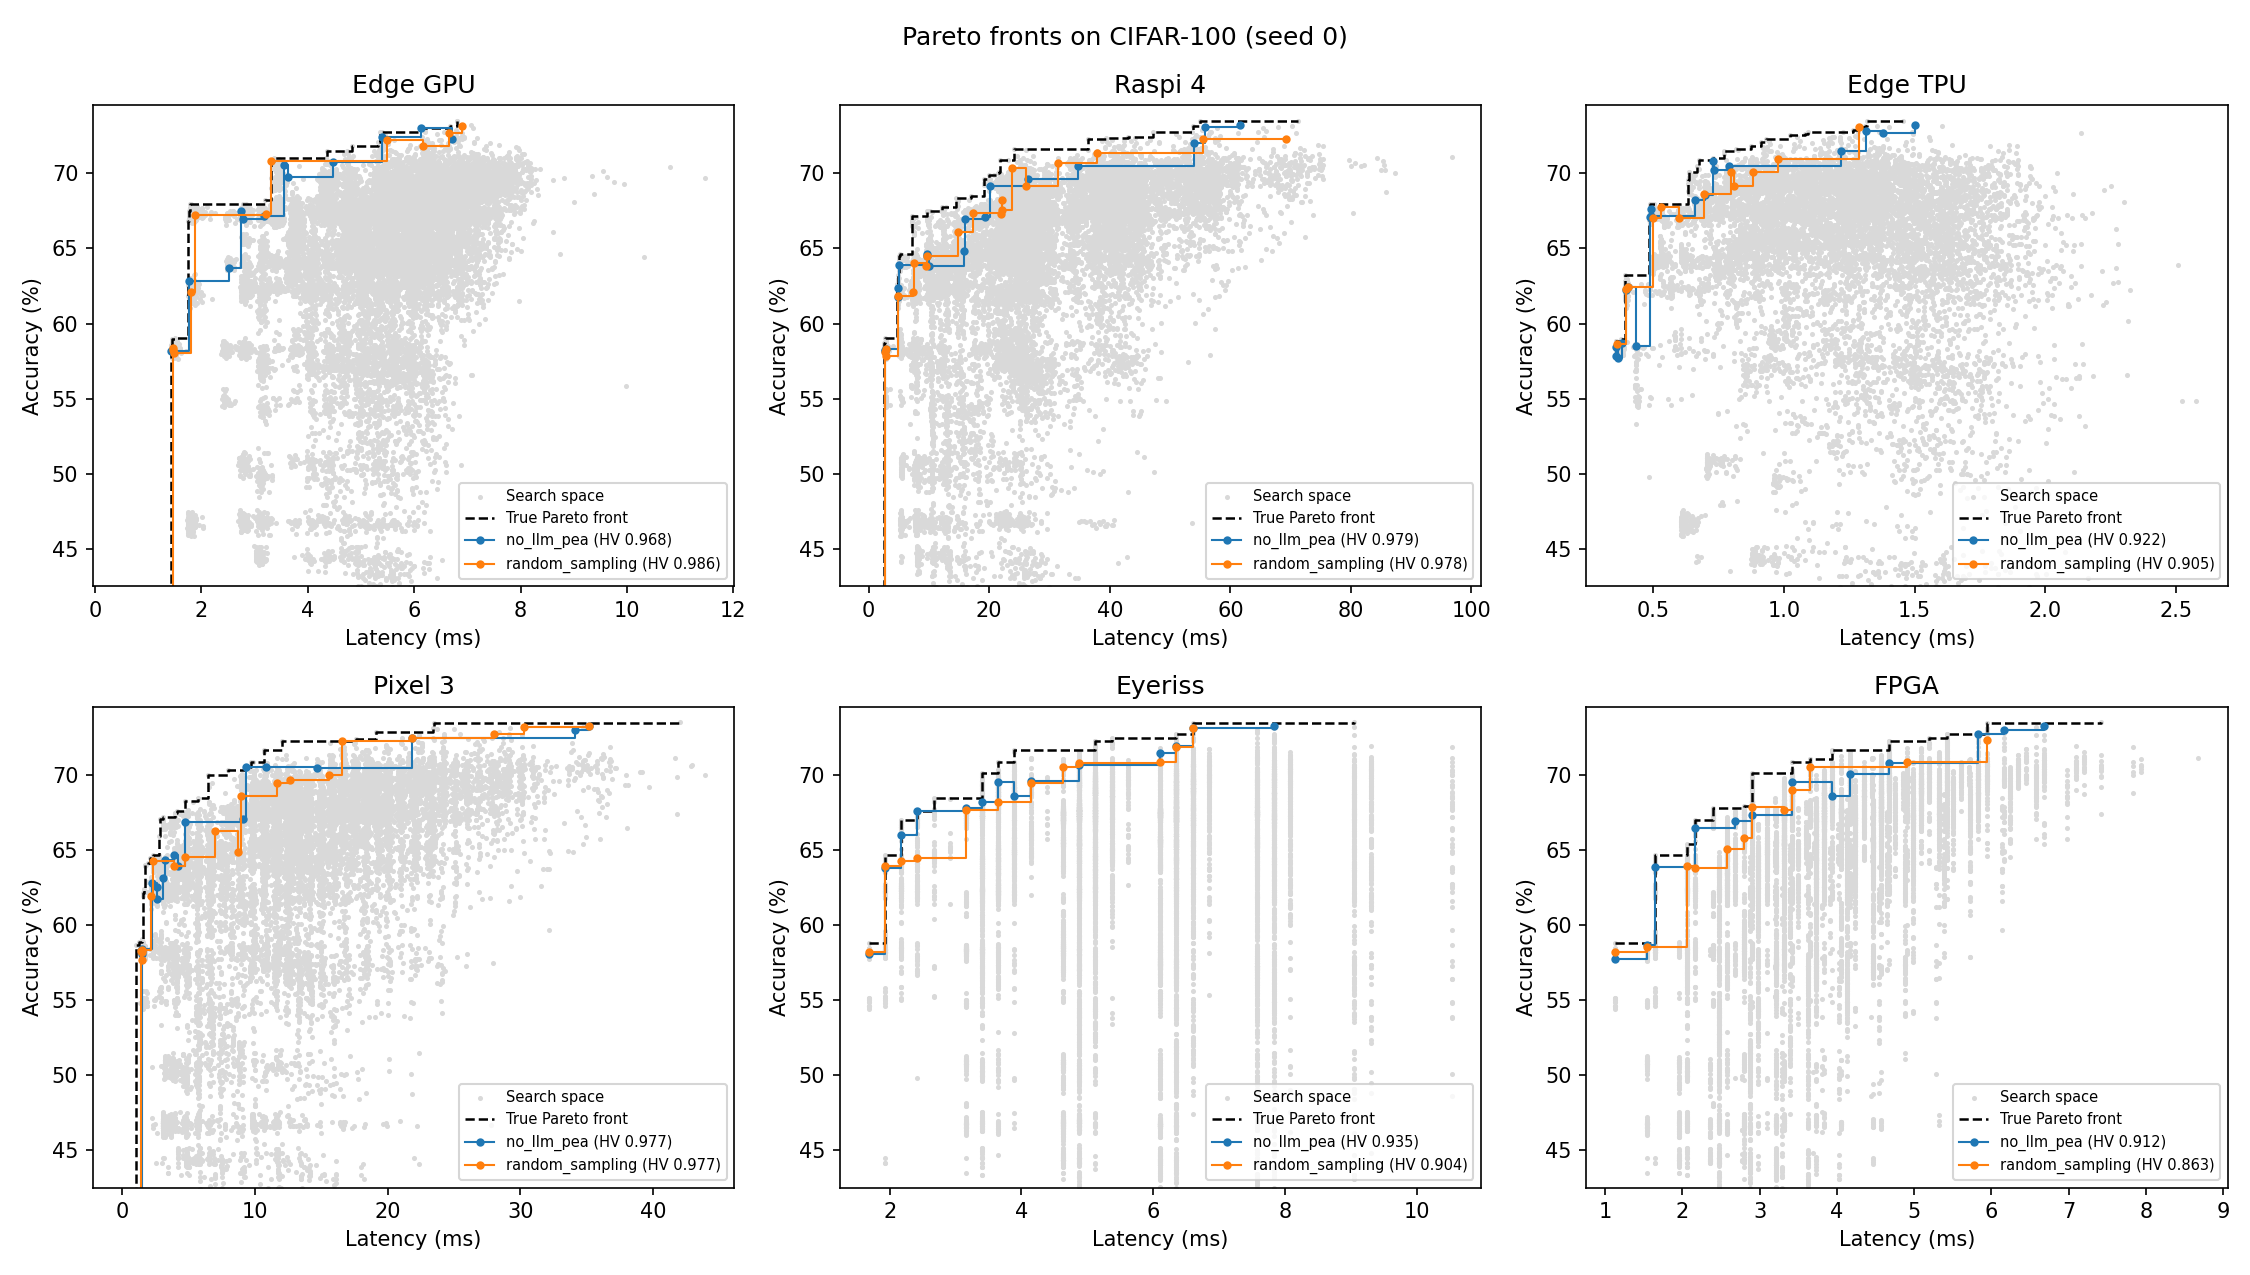
\includegraphics[width=\textwidth]{fronts_cifar100.png}
\caption{Non-LLM fronts on CIFAR-100 for all six devices (seed 0).}\label{fig:abl}
\end{figure}


\subsection{What the paper reports}
Table~\ref{tab:claims} lists the headline claims of the paper that this study checks. The paper also extends the method to a Vision Transformer space derived from AutoFormer on ImageNet-1k, with a different accuracy predictor; that part is not reproduced here.

\begin{table}[h]\centering\small
\caption{Headline claims of the LLM-NAS paper and where this study checks them.}\label{tab:claims}
\begin{adjustbox}{max width=\linewidth}
\begin{tabular}{p{3.4cm}p{8.2cm}p{3.0cm}}
\toprule
Claim & Value in the paper & Checked in \\
\midrule
Front quality (paper's Table~3) & HV of $0.931$--$0.997$ on CIFAR-10, $0.962$--$0.994$ on CIFAR-100 and $0.943$--$0.988$ on ImageNet16-120 across six devices, above LLMatic, FairNAS and PRP-NAS in every cell & the main paper, the main paper \\
Selected architectures (paper's Table~2) & CIFAR-10, four devices; for example 94.37\% at 4.35\,ms on Edge GPU, and a fastest model of 1.78\,ms at 89.18\% & the main paper \\
Ablation (paper's Table~5) & CIFAR-100, HV averaged over six devices: full model $0.978$; without partitioning $0.516$; partitioned evolutionary algorithm instead of the LLM $0.843$; Synflow instead of the ensemble $0.819$ & the main paper, Table~\ref{tab:abl} \\
Search cost (paper's Table~4) & 120 API calls and about 3 minutes per dataset and device, against 2--17 GPU-days for PRP-NAS-BA, DARTS, FairNAS and LLMatic & the main paper \\
\bottomrule
\end{tabular}
\end{adjustbox}
\end{table}


\subsection{Framework}
The implementation is a Python package, written with the assistance of an AI coding tool (Claude Code) and reviewed by us; every number in this paper is produced by it and can be regenerated from the archived run logs. It has the following properties, all motivated by the need to regenerate every number years later:
\begin{itemize}[nosep]
  \item \textbf{One configuration system.} \code{configs/base.yaml} holds every default, each tagged \code{[paper]} (stated in the paper) or \code{[assumed]} (our choice). Experiment files define a grid (datasets $\times$ devices $\times$ seeds) and named variants as overrides.
  \item \textbf{Content-addressed runs.} A run lives at \path{results/runs/<variant>-<hash8>/<dataset>/<device>/seed<k>/}, where the hash covers the effective configuration (excluding fields that cannot change results). A finished run is never recomputed, interrupted grids resume, and changing any setting creates a new directory rather than overwriting.
  \item \textbf{Replayable LLM calls.} Every prompt, response, token count and wall time is appended to \code{llm\_calls.jsonl}. Running with \code{llm.mode=replay} feeds the saved responses back and reproduces the run exactly (a mismatch counter must read zero); verified on the Qwen run, which replayed identically in 1.4\,s.
  \item \textbf{Provenance.} Each run records the git commit (with a dirty flag) that produced it.
  \item \textbf{Pluggable LLM backends.} Any OpenAI-compatible endpoint (GPT-4.1, OpenRouter, Ollama), Anthropic Claude, or an offline mock used only for tests.
  \item \textbf{Tests.} Unit and end-to-end tests run on synthetic data without the 2\,GB download, including searches with the mock backend and exact-replay checks.
\end{itemize}


\subsection{Data}
Three public sources were merged into one table per dataset (15{,}625 rows): HW-NAS-Bench v1.0 (latency); NAS-Bench-Suite-Zero \code{zc\_nasbench201.json} (13 ZC proxies and validation accuracy); and NATS-Bench \cite{nats} (200-epoch \emph{test} accuracy, which is what the paper's Table~2 reports, e.g.\ the 94.37\% CIFAR-10 optimum). NASLib encodes architectures with a different operator order and edge permutation from the NB201 string. The mapping (operators \code{[skip,none,conv3,conv1,pool]}, edge permutation $[0,1,3,2,4,5]$) was verified by matching validation accuracies on all 15{,}625 architectures.


\subsection{LLM co-evolution of knowledge and architectures}
In every generation and in every niche the LLM is called twice (Appendix~E of the paper). In \emph{Stage~1} it acts as an analyst: given the device and dataset, the niche definition and the current Pareto parents with their accuracy, latency and rationales, it is asked to identify operator or connection patterns that consistently help or hurt, to write them as rules of the form ``use/avoid \ldots\ because \ldots'', and to drop or revise earlier rules that the new evidence contradicts; its output is the updated knowledge base. In \emph{Stage~2} it acts as an architect: given the niche constraints, the parents with their metrics and the updated knowledge base, it produces new candidates, deciding for each whether to apply crossover (combine two parents) or mutation (modify one), describing which edges it changes, and justifying the change by its expected effect on accuracy and latency; the output is a list of JSON objects holding an identifier, the operation, the architecture code and the rationale. The candidates are evaluated at once, and their metrics and rationales feed Stage~1 of the next generation, which the authors call the co-evolution of prompts and architectures. Their example is a rule that average pooling costs latency for little accuracy gain, replacing an earlier rule that it always helps. The search runs for 10 generations with crossover probability $p_c=0.5$ and GPT-4.1 as the LLM, so one search makes $6\times10\times2=120$ calls. Algorithm~\ref{alg:llmnas} paraphrases the procedure.

\begin{algorithm}[t]
\caption{LLM-NAS, paraphrasing Algorithm~1 and Appendix~E of the paper.}\label{alg:llmnas}
\begin{algorithmic}[1]
\Require generations $G=10$, LLM $L$, niches $S_0,\dots,S_5$, latency table $l(\cdot)$
\State fit the accuracy predictor $M$ on a sample of architectures (offline, once)
\For{each niche $k=0,\dots,5$}
  \State sample an initial population from $S_k$, score each member with $(M(A),l(A))$ and keep the non-dominated ones as the archive $P_k$
\EndFor
\For{generation $g=1,\dots,G$}
  \For{each niche $k$ (independently)}
    \State \textbf{Stage 1:} $K_k\gets L(\cdot)$, given the device, dataset, niche $S_k$ and the parents from $P_k$ with their metrics and rationales
    \State \textbf{Stage 2:} choose parents from $P_k$; $\text{children}\gets L(S_k,\text{parents},K_k)$, each by crossover or mutation, with a rationale
    \For{each child $A$ that is valid, novel and inside $S_k$}
      \State $(z,l)\gets(M(A),l(A))$; add $A$ to $P_k$ and remove the members it dominates
    \EndFor
  \EndFor
\EndFor
\State \Return NonDominatedSort$\big(\bigcup_k P_k\big)$
\end{algorithmic}
\end{algorithm}

Several details of the paper matter for a reproduction. Its Algorithm~1 shows one child per niche per generation and omits Stage~1, whereas Appendix~E asks for $N_{\text{child}}$ children per call and describes both stages; it samples an initial population without giving its size; and it does not say how the knowledge base starts. Section~\ref{sec:assumed} records how we resolved these.


\subsection{Training-free evaluation}
No candidate is trained. Latency is a lookup in HW-NAS-Bench, which the paper describes as simulating rapid, noise-free hardware measurements. Accuracy is predicted by a surrogate: an XGBoost regressor that takes the 13 zero-cost proxies of NAS-Bench-Suite-Zero \cite{nbsz} as features, following that paper's ensemble strategy and trained once offline on a sample of architectures; the authors report a Spearman rank correlation of about 0.90 with the true accuracy. A search therefore costs the LLM calls and nothing else, which is the source of the paper's cost claim. the main paper compares the LLM operator with conventional operators on this same evaluator.


\subsection{Cost}
The paper reports 3 minutes and 120 API calls per search. Our GPT-4.1 run made 120 calls and took 8.6 minutes (about 4\,s per call, API latency included) and cost about \$0.85 at the measured token counts, so the paper's full Table-3 grid (18 settings, 3 seeds) would cost roughly \$46. Claude Opus~5.5 took 70.8 minutes (35\,s per call) and cost \$10.77, i.e.\ $12.7\times$ GPT-4.1: its adaptive thinking produced 450{,}669 output tokens, $6.7\times$ GPT-4.1's, and output tokens are billed at five times the input rate. The same grid with Claude at this setting would cost about \$580. The two local models carry no API fee but are slow on a 4\,GB laptop GPU: Qwen2.5-7B about 60--95\,s per call (124--191\,min per search over 18 searches) and DeepSeek-Coder-V2-16B about 30--90\,s per call (63--177\,min per search over 18 searches; its seed-0 search took 70.8\,min). By coincidence Claude and DeepSeek took the same total time (4249\,s each, confirmed by file timestamps; their per-call timing profiles are unrelated). No LLM here matched the 3\,minutes reported in the paper.


\subsection{Why hardware-aware search}
A network that is accurate is not necessarily one that runs well on a given device. Hardware-aware neural architecture search (HW-NAS) looks for architectures that trade task accuracy against a cost measured on the target hardware, such as latency or energy. The reason to measure, not to count operations, is that operation counts predict the cost poorly. MobileNet and NASNet have similar FLOPs (575M and 564M) but run in 113\,ms and 183\,ms on the same phone \cite{mnasnet}; a network with 19\% fewer multiply-accumulates was 29\% slower in practice \cite{netadapt}. On the six devices of HW-NAS-Bench, the Kendall rank correlation between FLOPs and latency ranges from $0.83$ on an FPGA down to $0.18$ on an Edge TPU \cite{hwnasbench}. The best network also differs by device: an architecture searched for an iPhone~X was $1.4\times$ faster there than one searched for a Samsung phone \cite{fbnet}.


\begin{table}[h]\centering\footnotesize
\caption{As the main paper with architectures below 80\% test accuracy removed from the true front and from all fronts. Devices without a degenerate cell (Edge TPU, Eyeriss, FPGA) are unchanged.}\label{tab:multidevicefloor}
\setlength{\tabcolsep}{2.5pt}
\begin{adjustbox}{max width=\linewidth}
\begin{tabular}{lccccccc}
\toprule
Method & Edge~GPU & Raspberry~Pi~4 & Edge~TPU & Pixel~3 & Eyeriss & FPGA & Mean \\
\midrule
GPT-4.1 & 0.752 & 0.875 & 0.902 & 0.895 & 0.896 & 0.839 & 0.860 \\
Claude Haiku~4.5 & 0.710 & 0.865 & 0.844 & 0.858 & 0.840 & 0.807 & 0.821 \\
Qwen2.5-7B & 0.781$\pm$0.106 & 0.827$\pm$0.047 & 0.845$\pm$0.050 & 0.833$\pm$0.011 & 0.787$\pm$0.035 & 0.819$\pm$0.035 & 0.815 \\
DeepSeek-Coder-V2 & 0.825$\pm$0.091 & 0.838$\pm$0.034 & 0.801$\pm$0.027 & 0.808$\pm$0.044 & 0.768$\pm$0.058 & 0.838$\pm$0.027 & 0.813 \\
\midrule
PEA & 0.870$\pm$0.052 & 0.901$\pm$0.033 & 0.921$\pm$0.020 & 0.895$\pm$0.027 & 0.908$\pm$0.019 & 0.913$\pm$0.017 & 0.901 \\
PEA with refilling & 0.922$\pm$0.039 & 0.922$\pm$0.023 & 0.942$\pm$0.015 & 0.912$\pm$0.016 & 0.919$\pm$0.015 & 0.919$\pm$0.020 & 0.923 \\
Random sampling & 0.911$\pm$0.055 & 0.903$\pm$0.010 & 0.933$\pm$0.011 & 0.894$\pm$0.025 & 0.895$\pm$0.028 & 0.904$\pm$0.019 & 0.907 \\
NSGA-II & 0.953$\pm$0.011 & 0.942$\pm$0.016 & 0.949$\pm$0.010 & 0.938$\pm$0.011 & 0.945$\pm$0.015 & 0.943$\pm$0.014 & 0.945 \\
Regularised evolution & 0.951$\pm$0.020 & 0.935$\pm$0.013 & 0.964$\pm$0.011 & 0.923$\pm$0.015 & 0.932$\pm$0.012 & 0.939$\pm$0.009 & 0.941 \\
\bottomrule
\end{tabular}
\end{adjustbox}
\end{table}

\begin{figure}[h]\centering
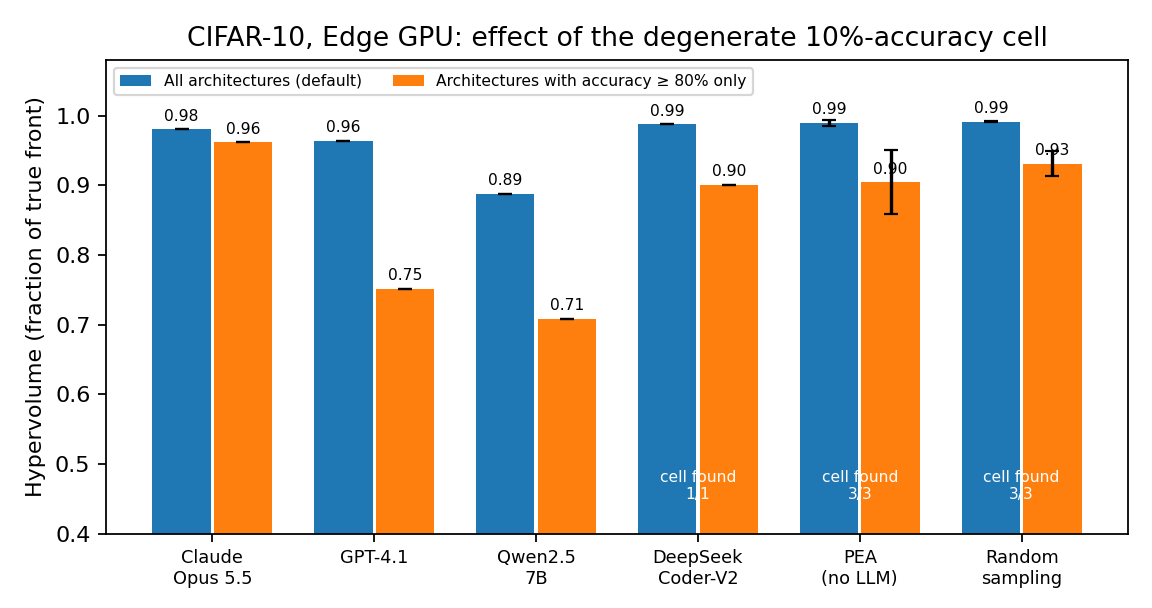
\includegraphics[width=0.85\textwidth]{hv_floor.png}
\caption{Hypervolume with and without the degenerate 10\%-accuracy architecture (error bars: sample s.d.\ over seeds, three for DeepSeek and Qwen and ten for the controls; GPT-4.1 and Claude Opus have one seed). Excluding it lowers every method, by 0.02 (Claude) to 0.21 (GPT-4.1), because the accuracy axis is re-spread; the direct bonus for including it is only 0.012--0.014 (controls and DeepSeek).}\label{fig:floor}
\end{figure}

\begin{figure}[!ht]\centering
\begin{adjustbox}{max width=\linewidth}
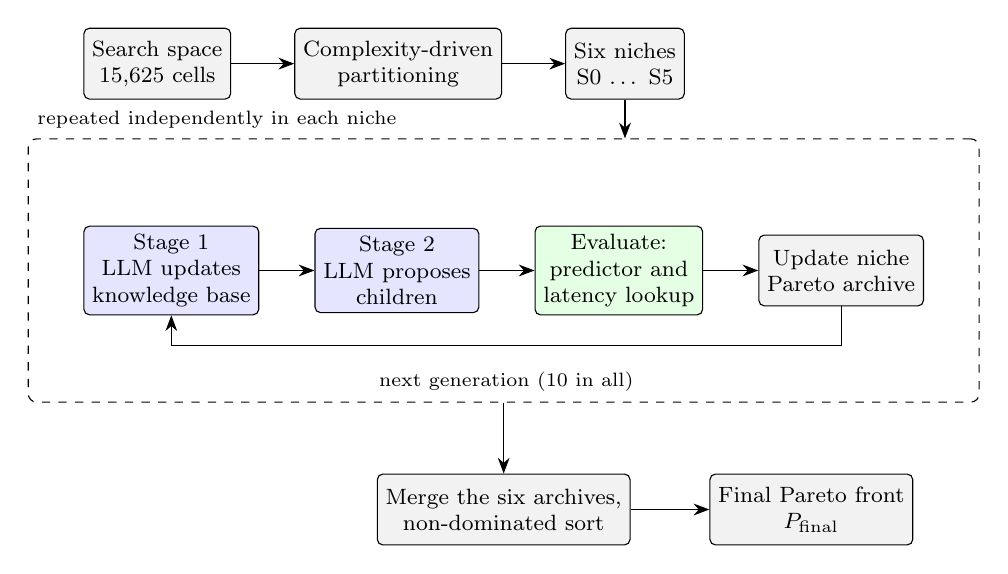
\begin{tikzpicture}[font=\footnotesize,>={Stealth[length=2mm]},
  box/.style={draw,rounded corners=2pt,align=center,fill=gray!10,inner sep=3pt,minimum height=9mm},
  llm/.style={box,fill=blue!10},
  ev/.style={box,fill=green!10}]
\node[box] (space) {Search space\\$15{,}625$ cells};
\node[box,right=8mm of space] (part) {Complexity-driven\\partitioning};
\node[box,right=8mm of part] (niches) {Six niches\\S0 \ldots\ S5};
\draw[->] (space)--(part); \draw[->] (part)--(niches);
\node[llm,below=16mm of space.south west,anchor=north west] (s1) {Stage 1\\LLM updates\\knowledge base};
\node[llm,right=7mm of s1] (s2) {Stage 2\\LLM proposes\\children};
\node[ev,right=7mm of s2] (eval) {Evaluate:\\predictor and\\latency lookup};
\node[box,right=7mm of eval] (arch) {Update niche\\Pareto archive};
\draw[->] (s1)--(s2); \draw[->] (s2)--(eval); \draw[->] (eval)--(arch);
\draw[->] (arch.south) -- ++(0,-5mm) -| (s1.south);
\path (s1.south) -- (arch.south) node[midway,yshift=-9mm,font=\scriptsize] {next generation (10 in all)};
\node[draw,dashed,rounded corners=3pt,fit=(s1)(s2)(eval)(arch),inner sep=7mm,inner ysep=11mm] (loop) {};
\node[font=\scriptsize,anchor=south west] at (loop.north west) {repeated independently in each niche};
\draw[->] (niches.south) -- (niches.south |- loop.north);
\node[box,below=9mm of loop] (agg) {Merge the six archives,\\non-dominated sort};
\node[box,right=10mm of agg] (front) {Final Pareto front\\$P_{\mathrm{final}}$};
\draw[->] (loop.south) -- (agg.north);
\draw[->] (agg)--(front);
\end{tikzpicture}
\end{adjustbox}
\caption{The LLM-NAS pipeline as described in the paper (our redrawing).}\label{fig:pipeline}
\end{figure}

\begin{figure}[h]\centering
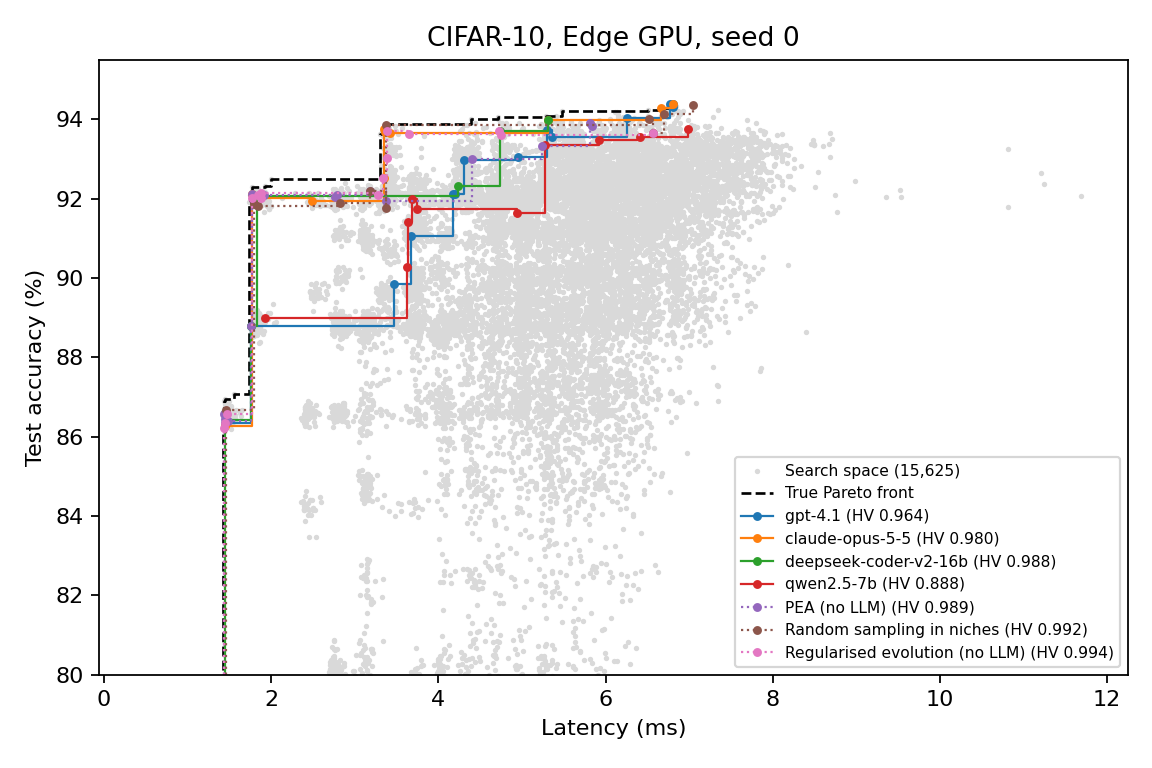
\includegraphics[width=0.8\textwidth]{cnn_fronts_edgegpu.png}
\caption{Final fronts on CIFAR-10 / Edge GPU (seed 0; of the controls, PEA, random sampling and regularised evolution are shown) against the true Pareto front. GPT-4.1 and Claude recover the 94.37\% optimum; DeepSeek's best is 93.99\% and Qwen's 93.77\%. Except for DeepSeek's, whose front also contains a degenerate 0.63\,ms / 10\% cell below the plotted range, all LLM fronts start at 1.4--1.9\,ms, while the true front extends to a degenerate 0.50\,ms / 10\% cell.}\label{fig:cnnfronts}
\end{figure}

\begin{table}[h]\centering\footnotesize
\caption{Pre-registered duplicate-fix test, Q1. Evaluated architectures $N$ and duplicate rate (share of all proposals that repeated an evaluated cell, retries included) for the reference GPT-4.1 searches and the two arms, CIFAR-10, one seed per device.}\label{tab:dupfixq1}
\setlength{\tabcolsep}{4pt}
\begin{adjustbox}{max width=\linewidth}
\begin{tabular}{l|ccc|ccc}
\toprule
 & \multicolumn{3}{c|}{$N$} & \multicolumn{3}{c}{Duplicate rate (\%)} \\
Device & Reference & Arm A & Arm B & Reference & Arm A & Arm B \\
\midrule
Edge GPU       & 129 & 231 & 166 & 44.6 & 47.1 & 38.8 \\
Raspberry Pi 4 & 161 & 241 & 165 & 40.4 & 49.6 & 38.3 \\
Edge TPU       & 141 & 244 & 140 & 34.6 & 42.7 & 30.8 \\
Pixel 3        & 151 & 245 & 170 & 40.4 & 48.4 & 38.8 \\
Eyeriss        & 140 & 247 & 179 & 52.5 & 50.5 & 31.2 \\
FPGA           & 148 & 251 & 161 & 43.8 & 51.7 & 37.5 \\
\midrule
Mean           & 145 & 243 & 164 & 42.7 & 48.3 & 35.9 \\
Pass mark      &     & $\ge265$ on all & & & $\le22.7$ & $\le32.7$ \\
\bottomrule
\end{tabular}
\end{adjustbox}
\end{table}

\subsection{Future work}\label{sec:future}
Ordered by cost and by how much each would change the conclusions:
\begin{enumerate}
  \item \textbf{Obtain the paper's HV/IGD convention from the authors} (reference point, normalisation, whether $S$ is the archive or all evaluated architectures, and whether degenerate cells such as the 0.50\,ms / 10\% architecture are on their true front) and re-score the archived runs. Zero cost; the replay logs make this a one-line change.
  \item \textbf{Report a floored hypervolume everywhere} (\code{compare-llms --min-acc}, extended to all datasets and devices with an appropriate floor) and re-run the CIFAR-100 ablation under it; this is also the cheapest way to see whether the PEA-versus-full-model gap in the paper's Table~5 survives.
  \item \textbf{GPT-4.1, three seeds, CIFAR-10 on all six devices} (6 devices $\times$ 3 seeds $\times$ 120 calls $\approx$ 2{,}160 calls, $\approx\$15$), then the CIFAR-100 and ImageNet16-120 slices to complete Table~3 (full grid $\approx\$46$). This gives the seed-to-seed spread of the paper's own model, which the local models suggest is large. Two more seeds of Claude Opus~5.5 on Edge GPU (about \$22) would show whether its first place under the floor is a model-capability effect or a single good search.
  \item \textbf{Complete the CIFAR-100 ablation} with the full-model and Synflow variants, so that Table~5 can be compared row by row (GPT-4.1 on six devices, about \$5 for one seed).
  \item \textbf{Remedies for proposal waste not yet tested.} The history list and re-prompting were tested in the main paper and did not help. Untested are schema-constrained decoding with the niche's operator counts enforced, which would remove out-of-niche proposals but not repeats; replacing the list of evaluated cells by a summary the model can use more easily (for example, the operators already tried on each edge); and the same arms with a stronger model and with more than one seed.
  \item \textbf{Sensitivity study on the assumed hyper-parameters} (children per call $\in\{2,4,8\}$, predictor $n_{\text{train}}\in\{200,1000,5000\}$, parents shown), reported with the alternative HV conventions.
  \item \textbf{Run the exploration-bias experiment} (the paper's Figures~1 and 9; implemented, 10--20 calls per device) to test the paper's motivating claim directly.
  \item \textbf{Cheaper thinking and more LLMs at a fixed budget.} Re-run Claude Opus~5.5 with \code{llm.effort=low} to measure how much of its advantage survives at a fraction of the \$10.77, then Claude Sonnet~5.5 and Haiku~4.5, GPT-4.1-mini and a 14B local model, to map the quality-versus-cost curve suggested by the Qwen / GPT-4.1 / Claude ordering.
  \item \textbf{Re-run a baseline} (e.g.\ a NAS-Bench-201 supernet or PRP-NAS if code is available) so that the quoted baseline numbers are on the same footing as ours.
  \item \textbf{Vision-Transformer experiment} (Section~4.4 of the paper), which needs an AutoFormer supernet, the ViT-Bench-101 predictor and latency profiling on a GPU.
\end{enumerate}


\subsection{Reproducibility and artefacts}
All code, configurations and run logs are provided as anonymised supplementary material. Benchmark data (2\,GB) is re-created by \code{python -m llmnas prepare-data}. The archived \path{results/runs/} directory (per run: \code{config.yaml}, \code{run.json}, \code{llm\_calls.jsonl}) is the evidence behind every number in this paper; \code{python -m llmnas report <experiment>} regenerates the tables and figures, and \code{--set llm.mode=replay} re-executes any LLM search without API access. A Colab notebook performs the same steps with data and results on Google Drive. Each run records the commit that produced it: the GPT-4.1 run used commit \code{1b5cf55}, the Qwen run and the non-LLM controls \code{bd5df23} (both 2 October 2026); neither commit changes the search or metric code relative to the other. The Claude run used commit \code{1474a23} (25 October 2026) and is one command, \code{python -m llmnas run claude\_cnn}; the DeepSeek run recorded \code{1474a23-dirty} because an untracked Modelfile was present at launch (no search or metric code differed); \code{python -m llmnas compare-llms} produces the side-by-side LLM table, with and without the accuracy floor. The tables of the main paper--the main paper are generated by \code{python -I report/paper\_numbers.py}, which uses the same scoring, and those of the main paper by \code{python -m llmnas dupfix}. The pre-registration, its two amendments and its outcome are in \code{PREREGISTRATION\_duplicate\_fix.md}; the paid arms ran on commit \code{3e2dd02} (23 November 2026) with the search code frozen in \code{754bc79}.
\paragraph{What other studies report.} Our finding is consistent with, though not proof of, the wider literature.
\begin{itemize}[nosep]
  \item The authors of CoLLM-NAS state that most existing LLM-based NAS methods face ``architectural invalidity, computational inefficiency, and inferior performance compared to traditional NAS'' \cite{collmnas}. Their remedy is a two-model collaboration with knowledge guidance, which suggests that a single prompted LLM, as in LLM-NAS, is not sufficient on its own.
  \item Yoshimura et al.\ report that LLM proposals ``are often biased toward a narrow set of patterns observed in their training data'' and assign coarse-level planning to a diversity-guided Bayesian algorithm, using the LLM only to fill in the remaining degrees of freedom \cite{llmtool}. This is the same remedy in spirit as the paper's partitioning, achieved by a conventional algorithm.
  \item In earlier, non-LLM work, uniform random search in a well-designed space was only slightly worse than evolution: 0.3 percentage points lower top-1 accuracy on CIFAR-10 and 0.1 on ImageNet \cite{hierarchical}. This is relevant because it shows that a strong random baseline is the standard that a new operator must beat.
  \item LLMatic does not rely on prompting alone: its authors report that LLMs struggle to conduct NAS directly through prompts, so it wraps LLM-generated variations in a quality-diversity algorithm, and it trains every candidate, which is why its search cost in Table~4 of the paper is the highest \cite{llmatic}.
\end{itemize}
We did not find a study that compares prompted-LLM search with strong evolutionary and random baselines under equal budgets and the same evaluator across several benchmarks. LLM-NAS does not provide one either; this is the gap that the controls in this paper begin to fill.


\paragraph{Relation to other work.} Filtering repeated candidates is common in LLM-driven search, but the studies we found report it differently. Work that generates network code removes near-duplicates by MinHash--Jaccard similarity and reports how many architectures were admitted \cite{khalid26,adhikari26}. A spiking-network search removes 30\% of raw LLM proposals as near-duplicates by a behavioural fingerprint \cite{zhao26spiking}. Program-evolution systems reject candidates by embedding similarity \cite{shinka}, or discard a duplicate and ask again up to a fixed number of attempts \cite{lyria}. None of these break duplicates down by where the repeated design came from, and they do not measure how the loss shrinks the evaluation budget relative to a baseline. The two LLM-based methods that report NAS-Bench-201 results do not analyse duplicates: GENIUS feeds every result back to GPT-4 and compares against random sampling after ten iterations \cite{genius}, and LLMatic generates 100 offspring per generation without a stated deduplication step \cite{llmatic}. The closest budget-matched comparison we found is in hyperparameter optimisation: an LLM advisor was overtaken by random search and Bayesian optimisation within a few evaluations, and its early lead came from a default configuration rather than from the LLM \cite{rodrigues26}. To our knowledge, this is the first exact count of duplicate LLM proposals in an enumerable NAS space, broken down by source, together with its effect on the evaluated budget. The remedies are known: rejecting and regenerating duplicates as evolutionary algorithms do \cite{mauldin84,lyria}, or showing the model its search history as OPRO does \cite{opro}. We do not claim them as contributions; the main paper tests whether they work here.


\paragraph{Where an LLM operator could still be justified.} The data above do not show that the LLM is useless, only that, on this benchmark, with this evaluator and this budget, it does not beat cheap alternatives. Four conditions under which it might do so are untested:
\begin{enumerate}[nosep]
  \item \emph{Expensive evaluations.} Here an evaluation costs about a millisecond (predictor plus lookup), so using fewer of them saves nothing and a second of random search is cheaper than any API call. If each evaluation meant training a network (hours), an operator that needed 30\% fewer evaluations would pay for its API cost. Our data show no such reduction, but the test was not run in that regime.
  \item \emph{Search spaces without a natural encoding.} NAS-Bench-201 has six categorical variables, for which random mutation is easy to write. In open-ended spaces (code, transformer variants, hardware-software co-design) writing a valid mutation operator is itself hard, and a text interface lets the LLM operate without one. The paper's Vision-Transformer experiment is of this kind; we did not reproduce it.
  \item \emph{Interpretability.} The knowledge base and the per-design rationales give a human-readable record of why designs were chosen. This is a real property that random operators lack. In our runs only the strongest model (Claude) produced rules backed by its own evidence; the others produced generic, sometimes self-contradicting rules, so the benefit depends on the model.
  \item \emph{Small spaces versus large spaces.} NAS-Bench-201 contains 15{,}625 architectures and our random baseline evaluates about 270 of them (1.7\%); in so small a space random search is a strong baseline. In spaces many orders of magnitude larger, a good prior could matter more. Whether the LLMs saw these benchmark tables during pre-training is unknown; if they did, the prior would be inflated rather than informative, and it is another reason to test on a held-out space.
\end{enumerate}


\paragraph{What the paper offers as justification.} The paper makes four arguments \cite{llmnas}. (i)~\emph{Cost}: supernet-based NAS needs GPU-days (Table~4 of the paper, per dataset and device on a V100: LLMatic 17 GPU-days, FairNAS 10, DARTS 4, PRP-NAS-BA 2), whereas LLM-NAS needs ``3\,mins (API calls)''. (ii)~\emph{No supernet, no training}: the LLM replaces the supernet-based sampler, and candidates are scored by zero-cost proxies. (iii)~\emph{Knowledge and feedback}: the LLM brings prior architectural knowledge and, through the co-evolved knowledge base, accumulates design rules from past evaluations, which the paper argues ``avoids random guesswork'' and improves efficiency. (iv)~\emph{Interface}: the operator needs only a textual description of the search space and returns a rationale for each design, so it does not require a hand-written mutation or crossover operator. The paper positions LLMs against two alternatives: supernet-based methods (OFA, FairNAS) and earlier LLM-driven search (LLMatic, which trains every candidate). Classical multi-objective evolutionary algorithms such as NSGA-II are cited as the natural fit for the problem, but no equal-budget evolutionary baseline using the same predictor appears in its comparison, apart from the PEA ablation (random operators inside the same framework).


\paragraph{Evidence 2: cost.} Table~\ref{tab:costcmp} puts the quality and cost of one search side by side.
\begin{table}[h]\centering\footnotesize
\caption{One search (120 LLM calls, or none) on CIFAR-10 / Edge GPU. Prices are list prices for the measured token counts. The local models ran on a 4\,GB laptop GPU; their rows are means over three seeds, the controls' over ten.}\label{tab:costcmp}
\begin{adjustbox}{max width=\linewidth}
\begin{tabular}{lcccc}
\toprule
Operator & HV (default) & HV ($\ge80\%$ acc.) & Cost & Wall time \\
\midrule
NSGA-II                              & $0.994\pm0.001$ & $0.953\pm0.011$ & \$0 & seconds \\
Regularised evolution                & $0.994\pm0.002$ & $0.951\pm0.020$ & \$0 & seconds \\
PEA with refilling                   & $0.991\pm0.003$ & $0.922\pm0.039$ & \$0 & seconds \\
Random sampling in niches            & $0.979\pm0.024$ & $0.911\pm0.055$ & \$0 & about 1\,s \\
Random operators, PEA                & $0.979\pm0.026$ & $0.870\pm0.052$ & \$0 & about 1\,s \\
GPT-4.1                              & 0.964 & 0.752 & \$0.85 & 8.6\,min \\
Claude Haiku~4.5                     & 0.913 & 0.710 & \$1.62 & 43\,min \\
Claude Opus~5.5                      & 0.980 & 0.961 & \$10.77 & 71\,min \\
Qwen2.5-7B (local)                   & $0.949\pm0.053$ & $0.781\pm0.106$ & \$0 (electricity) & 145\,min \\
DeepSeek-Coder-V2-16B (local)        & $0.983\pm0.008$ & $0.825\pm0.091$ & \$0 (electricity) & 125\,min \\
\bottomrule
\end{tabular}
\end{adjustbox}
\end{table}
Across six devices the GPT-4.1 searches cost \$0.80--0.88 each and the Haiku searches \$1.44--1.62. The non-LLM controls cost nothing and finish in about a second, which is more than $400\times$ faster than the fastest LLM search. A user who accepts the zero-cost evaluator therefore pays between \$0.85 and \$10.77, and between 8 and 150 minutes, per search for an operator that, on this benchmark, does not reach a better front. The only configuration ahead of the controls in our data is Claude Opus~5.5 under the 80\% floor, at the highest price; it is above every control mean but within the range of individual control seeds, and it rests on a single search (the main paper).


\paragraph{What would settle the question.} Run the framework with (a)~Bayesian optimisation with the same predictor and budget, in addition to the NSGA-II and regularised-evolution baselines reported here; (b)~at least three seeds for every LLM, as done here for the two local models; (c)~a larger, non-tabular search space; and (d)~a setting where each evaluation is a short training run. If the LLM operator reaches the same front with markedly fewer evaluations in (d), the cost argument becomes valid. Until then the more defensible reading of the paper's cost saving is that it comes from the zero-cost predictor, and that the LLM operator contributes interpretability and interface flexibility rather than a measurable gain in front quality on HW-NAS-Bench.


\section{Glossary of terms and formulas}

\begin{description}[style=nextline,leftmargin=0pt,itemsep=3pt]

\item[Architecture code (NB201).] A 6-tuple $(a,b,c,d,e,f)\in\{0,\dots,4\}^6$ giving the operator on each edge of the 4-node cell in the order $n_1{\leftarrow}n_0,\ n_2{\leftarrow}n_0,\ n_2{\leftarrow}n_1,\ n_3{\leftarrow}n_0,\ n_3{\leftarrow}n_1,\ n_3{\leftarrow}n_2$, with $0$=\code{none}, $1$=\code{skip\_connect}, $2$=\code{nor\_conv\_1x1}, $3$=\code{nor\_conv\_3x3}, $4$=\code{avg\_pool\_3x3}.

\item[Configuration hash.] SHA-1 (first 8 hex digits) of the canonical JSON of a run's effective configuration, excluding fields that cannot affect results. Identical settings map to the same run directory.

\item[Crossover / mutation.] Evolutionary operators. Uniform crossover copies each gene from parent $A$ or $B$ with probability $\tfrac12$; mutation changes the operator on one edge.

\item[Exploration bias / mode collapse.] The tendency of a generative model to repeatedly propose a narrow family of outputs; LLM-NAS's motivation for niching.

\item[Hypervolume (HV).] For a set $S$ of points in $m$-objective space (minimisation) and a reference point $r$ dominated by all of $S$,
\[
\HV(S,r)=\lambda\Big(\bigcup_{s\in S}[s_1,r_1]\times\cdots\times[s_m,r_m]\Big),
\]
the Lebesgue measure of the dominated region. We report the ratio $\HV(S,r)/\HV(P^\ast,r)$ after min--max normalising each objective by the ideal and nadir points of the true front $P^\ast$, with $r=(1.1,1.1)$. In two dimensions it is computed by sorting the front by latency and summing rectangles.

\item[Inverted generational distance (IGD).]
\[
\IGD(S,P^\ast)=\frac{1}{|P^\ast|}\sum_{p\in P^\ast}\min_{s\in S}\lVert p-s\rVert_2,
\]
the mean distance from each true-front point to its nearest discovered point (normalised objectives). Lower is better; zero iff $S\supseteq P^\ast$.

\item[Isotonic regression.] Monotone non-decreasing least-squares fit; used to map Synflow scores to the accuracy scale without changing their ranking.

\item[Knowledge base (co-evolve).] A list of natural-language rules of the form ``use/avoid \ldots because \ldots'' that the LLM rewrites after each generation from the previous cycle's results and that is injected into the next generation prompt.

\item[Min--max normalisation.] $\tilde{x}_j=(x_j-\min_j)/(\max_j-\min_j)$ per objective $j$, with the extremes taken over the true front, so that normalised objectives lie in $[0,1]$ on the front.

\item[NAS-Bench-201 / NATS-Bench / HW-NAS-Bench / NAS-Bench-Suite-Zero.] Tabular benchmarks. NB201 (= NATS-Bench topology space) gives trained accuracy for all 15{,}625 cells on CIFAR-10/100 and ImageNet16-120; HW-NAS-Bench adds latency and energy on six devices (measured on four, simulator-estimated on Eyeriss and the FPGA); NAS-Bench-Suite-Zero adds 13 zero-cost proxy scores per architecture.

\item[Niche (partitioning).] A disjoint subset of the search space defined by the number of $3{\times}3$ convolutions (Table~1 of the paper). Each niche keeps its own Pareto archive; archives are merged by non-dominated sorting at the end.

\item[Pareto dominance / front.] For minimisation, $a\preceq b$ iff $a_j\le b_j\ \forall j$ and $a_j<b_j$ for some $j$. The Pareto front is the set of non-dominated points; the \emph{true front} $P^\ast$ is the front of all 15{,}625 architectures (excluding the Edge TPU architectures that failed compilation).

\item[NSGA-II.] Non-dominated sorting genetic algorithm II \cite{deb02}: parents are chosen by Pareto rank and crowding distance, children by crossover and mutation. Here it runs inside each niche with the same predictor and regenerates rejected children until 270 architectures have been evaluated.

\item[PEA (partitioned evolutionary algorithm).] The paper's ``without LLM operator'' ablation: the same niches, archives and budget, with random mutation and crossover in place of the LLM.

\item[PEA with refilling.] PEA in which a child that is rejected (repeated, invalid or without latency) is redrawn, up to 50 times, and then replaced by a random unevaluated cell of the niche, so that the budget of 270 evaluations is always filled.

\item[Pre-registration.] A protocol that fixes the questions, arms, measures, decision rules and expected result of an experiment before its results exist, so that the analysis cannot be adapted to them. Amendments are allowed only before the results and are dated.

\item[Regularised (aging) evolution.] Tournament selection with removal of the oldest member of the population rather than the worst \cite{real19}; here run inside each niche with the same predictor and budget as NSGA-II.

\item[Replay.] Re-execution of a search with LLM responses taken from the saved call log instead of the API; must reproduce the original run exactly (mismatch counter 0).

\item[Seed.] Integer fixing a run's pseudo-random choices (initial population, predictor training sample, parent selection, crossover/mutation assignment, and the LLM sampling hint). Different seeds give independent repeats; results are reported as mean $\pm$ standard deviation over seeds.

\item[Sign-flip test.] An exact permutation test on the per-device differences between two methods: the observed mean difference is compared with the means obtained by flipping the signs of the differences in all $2^6=64$ ways. With six devices its smallest one-sided $p$ is $1/64=0.016$.

\item[Spearman / Kendall rank correlation.] $\rho=1-\frac{6\sum d_i^2}{n(n^2-1)}$ over rank differences $d_i$ (Spearman); $\tau=\frac{C-D}{\binom{n}{2}}$ over concordant and discordant pairs (Kendall). Used to validate the predictor against ground truth.

\item[Usable proposal rate.] Fraction of LLM (or operator) proposals that parse, satisfy the niche constraint and are not duplicates of already-evaluated architectures; the remainder consume budget without producing an evaluation.

\item[XGBoost.] Gradient-boosted decision-tree regressor; here 500 trees of depth 6, learning rate 0.05, trained on the 13 ZC proxies.

\item[Zero-cost (ZC) proxy.] A score computed from an untrained network (one forward/backward pass or less) that correlates with trained accuracy, e.g.\ \code{synflow}, \code{snip}, \code{grasp}, \code{fisher}, \code{jacov}, \code{nwot}, \code{zen}, \code{epe\_nas}, \code{grad\_norm}, \code{l2\_norm}, \code{plain}, \code{params}, \code{flops}.
\end{description}
\bibliographystyle{plainnat}
\bibliography{refs}
\end{document}
